\section{Evaluation of the Approaches and Scalability}
\label{sec:eval}

\subsection{Test setup}

All measurements come from the automated test scripts in the repository: single runs on 18
November 2026 (the numbers quoted in Section~\ref{sec:threats}) and repeated runs on 21 November
(Section~\ref{sec:repeat}).
Everything runs on one VM (4 vCPUs, 7.7~GiB RAM) as Incus containers: the two k3s nodes, the
Wazuh manager (4.14), the central Prometheus (2.53), the mail and DNS servers, and the load
generators. Locations are therefore \emph{logical}: dc1 and dc2 share the same CPU and disk, so
absolute numbers are lower bounds and the trends are what matters.

The scalability test uses three load-generator containers with 8 workers each, 20~s per phase, in
a closed loop (each worker sends its next request when the previous one returns). The Wazuh agents
are stopped during this test so the DoS rule does not block the load generators; it measures
capacity, not defence.

\subsection{Functional properties of the main deployment}

The cluster test checks every property of the architecture on k3s and passed 40/40 checks: both
nodes ready and labelled with their location; every Deployment available, each location's pods on
its own node, all images from the private registry; one registry entry per pod (pod addresses, both
dc1 and dc2) with the node name in the ID; readings accepted by the ingestion pod of each location;
the real client address in the pod's log; registry and storage not exposed; every service scraped
and the per-location aggregates federated centrally; both node agents active and a pod's access log
reaching the manager with the pod's ID; and self-healing: a deleted ingestion pod was replaced, the
new pod registered itself, and the health checker removed the old entry 15.8~s after the new one
registered.

\subsection{Horizontal scaling across locations}

Table~\ref{tab:scale} compares one instance (dc1) with two (dc1 and dc2) under the same load.

\begin{table}[ht]
\centering\small
\caption{Throughput and p95 latency with one and two instances.}
\label{tab:scale}
\begin{tabular}{@{}l rrr rr@{}}
\toprule
 & \multicolumn{3}{c}{throughput (req/s)} & \multicolumn{2}{c}{p95 (ms)} \\
\cmidrule(lr){2-4}\cmidrule(lr){5-6}
Service, platform & 1 inst. & 2 inst. & speed-up & 1 inst. & 2 inst. \\
\midrule
ingestion, k3s   & 85.8  & 114.8 & 1.34$\times$ & 426 & 475 \\
analytics, k3s   & 119.4 & 133.6 & 1.12$\times$ & 285 & 383 \\
ingestion, Incus & 189.9 & 184.3 & 0.97$\times$ & 199 & 540 \\
analytics, Incus & 194.3 & 207.9 & 1.07$\times$ & 175 & 234 \\
\bottomrule
\end{tabular}
\end{table}

Adding an instance helps little, and the reason is visible in the storage metrics: on Incus storage
wrote 198 readings/s with one ingestion instance and 184.7/s with two. Every write goes to one
SQLite storage, so a second ingestion instance only moves the bottleneck. Analytics only reads and
scales slightly better. Since both locations share one physical host, a second instance also
competes for the same CPU; these numbers cannot separate the two effects. During the repeated
runs analytics used up to 436 millicores of its 500-millicore limit and storage up to 350, so the
pods were close to their own CPU limits as well. Section~\ref{sec:repeat} shows how noisy these
measurements are.

\subsection{Registry growth}

The registry was filled with 0, 100, 500 and 2000 fake instances spread over 2 countries,
3 regions, 4 data centres and 5 racks (Figure~\ref{fig:registry}). On Incus, registration ran at
747--851 per second, and a filtered lookup stayed under 2~ms at the median (3.4~ms p95) with 2000
instances. The unfiltered \code{/services} response grows linearly to 404~kB, while a query for one
data centre returns 17~kB and for one rack 3.4~kB: filtering by location keeps discovery cost
proportional to the part of the system a client cares about. On k3s, where the benchmark runs
through the cluster network, 2000 instances gave 298 registrations/s and 4.1~ms (p50) / 38.7~ms
(p95) lookups.

\begin{figure}[ht]
\centering
% Figure 5: registry growth (Incus run, evidence/scale/3-registry.txt; FACTS.md section 9.6).
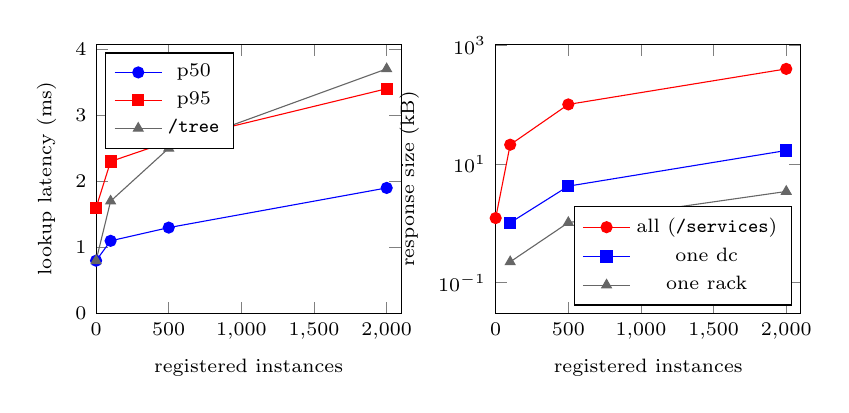
\begin{tikzpicture}
\begin{axis}[
  name=lat, width=0.45\textwidth, height=5cm,
  xlabel={registered instances}, ylabel={lookup latency (ms)},
  xmin=0, xmax=2100, ymin=0, legend pos=north west, legend style={font=\scriptsize},
  tick label style={font=\scriptsize}, label style={font=\scriptsize},
  scaled x ticks=false, xtick={0,500,1000,1500,2000}]
\addplot[mark=*, blue] coordinates {(0,0.8) (100,1.1) (500,1.3) (2000,1.9)};
\addlegendentry{p50}
\addplot[mark=square*, red] coordinates {(0,1.6) (100,2.3) (500,2.6) (2000,3.4)};
\addlegendentry{p95}
\addplot[mark=triangle*, black!60] coordinates {(0,0.8) (100,1.7) (500,2.5) (2000,3.7)};
\addlegendentry{\texttt{/tree}}
\end{axis}
\begin{axis}[
  at={(lat.east)}, anchor=west, xshift=12mm,
  width=0.45\textwidth, height=5cm,
  xlabel={registered instances}, ylabel={response size (kB)},
  ymode=log, ymin=0.03, xmin=0, xmax=2100, legend pos=south east, legend style={font=\scriptsize},
  tick label style={font=\scriptsize}, label style={font=\scriptsize},
  scaled x ticks=false, xtick={0,500,1000,1500,2000}]
\addplot[mark=*, red] coordinates {(0,1.226) (100,21.209) (500,101.473) (2000,403.593)};
\addlegendentry{all (\texttt{/services})}
\addplot[mark=square*, blue] coordinates {(100,1.024) (500,4.240) (2000,16.950)};
\addlegendentry{one dc}
\addplot[mark=triangle*, black!60] coordinates {(100,0.224) (500,1.028) (2000,3.449)};
\addlegendentry{one rack}
\end{axis}
\end{tikzpicture}

\caption{Registry with a growing number of instances (Incus run). Left: lookup latency and
\code{/tree}; right: response size of an unfiltered vs location-filtered query (log scale).}
\label{fig:registry}
\end{figure}

\subsection{Monitoring bandwidth by location}

One full scrape of an instance is 7--15~kB (registry 14.6~kB, storage 9.3~kB, ingestion 7.2~kB,
analytics 7.1~kB). A central Prometheus federating every raw series from the site Prometheus would
transfer 326.5~kB per scrape on Incus (10.8~kB gzip) and 403.6~kB on k3s; federating only the
\code{location:*} aggregates transfers 2.8~kB on Incus (0.4~kB gzip) and 2.9~kB on k3s, i.e.\
0.7\% of the raw federation. The per-location view still answers the operator's first question
(how many instances, how much traffic and errors, which latency in each data centre) and the
detail stays in the site Prometheus.

\subsection{Correlation and root cause}

Stopping storage produced several symptoms and one diagnosis (Table~\ref{tab:rootcause}). The
correlation rule named storage as root cause and did not blame the network, the registry dropped
the dead instance, and the alert cleared after recovery. The longer times on k3s are consistent with how
Kubernetes discovery works: a pod scaled to zero disappears from service discovery instead of reporting
\code{up == 0}, and its address stops answering, so each health check waits for its timeout.

\begin{table}[ht]
\centering\small
\caption{Root-cause test: storage stopped.}
\label{tab:rootcause}
\begin{tabular}{@{}l c c@{}}
\toprule
 & k3s & Incus \\
\midrule
\code{SSLERootCauseStorageDown} firing after & 43.4~s & 11.3~s \\
registry removed storage after & 54.1~s & 20.8~s \\
symptoms correlated (Prometheus alerts + Wazuh 5xx events) & 4 + 4 $\to$ 1 & 3 + 3 $\to$ 1 \\
alert cleared after restart & 7.1~s & 10.8~s \\
\bottomrule
\end{tabular}
\end{table}

\subsection{Repeated runs}
\label{sec:repeat}

Each k3s test was repeated five times back to back (scalability three times) to see how stable the
single-run numbers are (Table~\ref{tab:repeat}).

\begin{table}[ht]
\centering\small
\caption{Repeated runs on k3s (21 November): mean $\pm$ standard deviation and range.}
\label{tab:repeat}
\begin{tabular}{@{}l l r@{}}
\toprule
Test & quantity & mean $\pm$ sd (min--max), runs \\
\midrule
DNS hijack & alert after hijack & 0.12 $\pm$ 0.04~s (0.1--0.2), 5 \\
           & zone restored after & 0.28 $\pm$ 0.08~s (0.2--0.4), 5 \\
           & exposure seen by client & 0~s in all 5 \\
Junk email flood & first \rid{100222} alert & 1.8 $\pm$ 0.7~s (1.2--2.7), 5 \\
                 & source blocked after & 3.0 $\pm$ 2.5~s (1.5--7.3), 5 \\
Root cause & \code{SSLERootCauseStorageDown} firing & 40.9 $\pm$ 2.6~s (38--44), 5 \\
           & registry removed storage & 52.7 $\pm$ 2.2~s (49.6--54.9), 5 \\
           & alert cleared after restart & 5.3 $\pm$ 2.5~s (1.5--7.1), 5 \\
DoS & first \rid{100210} alert & 1.8, \emph{none}, 17.4, 1.6, 1.8~s (per run) \\
    & legitimate success, mitigated & 100, 0, 38, 100, 100\,\% (per run) \\
Scalability & ingestion speed-up (2 vs 1) & 0.37, 1.37, 1.27$\times$ (per run) \\
            & analytics speed-up & 5.66, 1.16, 1.22$\times$ (per run) \\
            & \code{location:*} share of raw federation & 0.71 $\pm$ 0.01\,\%, 3 \\
            & registry lookup with 2000 instances & p50 4.4 $\pm$ 0.6~ms, p95 47.5 $\pm$ 10.4~ms, 3 \\
\bottomrule
\end{tabular}
\end{table}

DNS restoration, the mail flood response, the root-cause diagnosis and the monitoring bandwidth
are stable. The DoS defence is not. In three of five runs the attackers were blocked within about
3~s and the legitimate client got 100\% of its requests through. In run~2 the analytics pod
completed \emph{no} request during the mitigated phase, so nothing was logged and Wazuh detected
nothing: the extreme case of the logging-on-completion weakness described in
Section~\ref{sec:threats}. Run~3 started while the service was still overloaded (its baseline
already failed), and detection took 17.4~s. The defence therefore depends on the attacked service
staying responsive enough to log the attack. The root-cause test also failed one of its own checks
in four runs because the previous run's symptom alert, computed over a one-minute window, had not
cleared yet; the diagnosis itself was correct in all five.

The scalability results vary too much to support a speed-up figure. Runs 2 and 3 agree (ingestion
1.37$\times$ and 1.27$\times$, analytics 1.16$\times$ and 1.22$\times$), but in run~1 the one-instance
analytics phase reached only 7.4~req/s, and at the end of that run the registry pod was killed by
its liveness probe (exit 137) after the 2000-instance benchmark, presumably because checking 2000 unreachable instances kept it
too busy to answer \code{/health} in time. The single-run speed-ups in
Table~\ref{tab:scale} should be read as indicative only.

\paragraph{Monitoring cost.} During the repeated scalability runs (samples every 5~s), the
in-cluster Prometheus used at most 44 millicores of CPU and 51--109~MiB of memory, with about 2\,200
active series; the central Prometheus container used 59--143~MiB. The Wazuh manager container used
2.0--2.6~GiB, by far the largest share of the monitoring and security stack on this host.

\subsection{SIEM throughput per node}

We wrote synthetic access-log lines on one k3s node at increasing rates for 30~s each and counted
how many became alerts at the manager and how late (log timestamp to alert timestamp). Each line
used a different source address, so no active response was triggered. Up to 500 lines/s every line
became an alert within about 2~s; above that the node's agent delivered at most about 590 events/s,
lost the rest and logged \emph{Agent buffer is full: Events may be lost}
(Table~\ref{tab:eps}). The cause is the agent's client buffer, configured at 500 events per second
with a 5000-event queue. Because one agent serves a whole node, a flood of more than about 500
logged requests per second on one node \emph{blinds the SIEM for every pod on that node}: the
first 15 requests still trigger \rid{100210}, but other events from the same node (for example
5xx errors from an unrelated pod) can be lost or arrive 11--15~s late. We did not measure the
manager's own limit, which a higher agent limit would expose.

\begin{table}[ht]
\centering\small
\caption{Wazuh pipeline from one k3s node: delivered alerts and latency per log rate (30~s each).}
\label{tab:eps}
\begin{tabular}{@{}rrrrrr@{}}
\toprule
lines/s & written & alerts & lost & p50 latency & p95 latency \\
\midrule
100  & 2\,884  & 2\,884  & 0\%    & 1.1~s  & 1.8~s \\
250  & 7\,499  & 7\,499  & 0\%    & 1.1~s  & 1.5~s \\
500  & 14\,999 & 14\,999 & 0\%    & 2.3~s  & 3.7~s \\
1000 & 29\,996 & 17\,777 & 40.7\% & 11.2~s & 12.1~s \\
2000 & 59\,992 & 16\,900 & 71.8\% & 11.5~s & 15.2~s \\
\bottomrule
\end{tabular}
\end{table}

\subsection{Scaling limits of each component}

\begin{itemize}
  \item \textbf{Storage} is a single SQLite writer: the measured bottleneck. Sharding by location or a
        replicated database is required before more ingestion instances help.
  \item \textbf{Registry} is a single in-memory process. Lookups stay fast, but the health checker
        pings every instance one after another (O($N$) per sweep, plus a 2~s timeout per dead
        instance), and unfiltered queries grow linearly. A registry per location, with the
        hierarchy delegated like DNS zones, would bound both.
  \item \textbf{Prometheus} is one server per site plus a central one; federation of aggregates keeps
        the central load proportional to the number of locations. At our size it is cheap (at most
        44 millicores and about 100~MiB for about 2\,200 series); its cost grows with the number of
        series, i.e.\ with instances and label combinations, which is why no client-controlled value
        is used as a label.
  \item \textbf{Wazuh} is a single manager. One agent per node instead of per pod keeps the number of
        agents proportional to machines, not pods, and avoids enrolling a new agent at every
        restart. The binding limit, however, is per agent (Table~\ref{tab:eps}).
  \item \textbf{Shared host.} All nodes share one disk: when free space fell below 5\%, the kubelet
        evicted every pod and blocked scheduling on both nodes. In a real multi-site deployment
        this failure would stay local to one site.
  \item \textbf{Operations.} After a reboot of the VM the Wazuh manager failed to start (its start-up
        timed out on the busy host) and nothing alerted on it: the SIEM was silently down until we
        noticed missing alerts. The stock service allows 45~s to start and never retries; we added a
        systemd override (5~min, restart on failure). Monitoring the SIEM itself (an \code{up}
        check on the manager) would still be needed to notice such a failure.
\end{itemize}
